\newpage
\section{Заключение}
	Все известные алгоритмы перечисления объектов теории узлов работают похожим образом: сначала каким-то образом генерируются
	все ``интересные'' диаграммы исследуемых объектов, затем с помощью определенных инвариантов и хеш-таблиц из полученного
	множества диаграмм удаляются повторы, соответствующие одному и тому же объекту. Например, в процессе перечисления альтернированных
	зацеплений в \cite{Rankin2002_1, Rankin2002_2, Rankin2002_3} для генерации диаграмм использовались локальные преобразования,
	как на \figureref{figure:surgeries}, а удаление дубликатов производилось с помощью введенного авторами полного инварианта
	``Master Array''.
	\begin{figure}[ht]
		\centering
		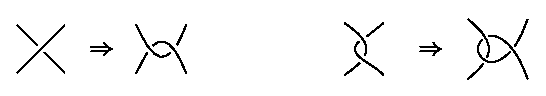
\includegraphics{c/surgeries.eps}
		\caption{Локальные преобразования\label{figure:surgeries}}
	\end{figure}

	Очевидным недостатком такой схемы являются необходимость поддерживать хеш-таблицу очень больших размеров и выполнять поиск
	по ней. Также часто возникает проблема с тем, что доля заведомо бесполезной работы с увеличением размера объектов возрастает
	экспоненциально, так как экспоненциально растет доля повторяющихся диаграмм. Предложенный в данной работе тип алгоритмов
	свободен от подобного рода проблем. Перебор проекций в Главе~\ref{section:projections} вообще не требует хранения уже
	полученных им объектов, а алогоритм генерации альтернированных $k$-танглов из Главы~\ref{section:alternating} не требует
	поиска и хранит только малую часть сгенерированного. Доля лишней работы растет не более чем линейно с ростом максимального
	числа концов.

	Еще одним достоинством предложенной схемы является широкая возможность ее обобщения. В качестве примера, легко понять как
	приспособить ее для генерации полимино, или диаграмм альтернированных зацеплений, или, возможно, самих альтернированных
	зацеплений.

	Вероятным следующим шагом могло бы явится обобщение алгоритма на неальтернированные $k$-танглы, впрочем в этом случае такое
	свойство, как отсутствие поисковых запросов по уже сгенерированным объектам, скорее всего не удастся сохранить.

	Реализации на языке C++ приведенных алгоритмов можно найти по адресу \uline{http://code.google.com/p/tanglenum/}.
